\documentclass[12pt]{article}
\usepackage{lingmacros}
\usepackage{tree-dvips}
\usepackage{datetime}
\usepackage{color}
\usepackage{graphicx}
\usepackage{cite}
\graphicspath{ {images/} }
\title{Master thesis proposal}
\author{Ion Madrazo Azpiazu}
\date{\today}
\begin{document}


\maketitle
\section{Introduction}

Reading is an important skill of not only in the educational context, but in daily tasks. People that get good understanding from the texts they read, tend to take better decisions when they face medical or educational problems, which can lead to better career opportunities in the future. Studies\cite{medicalReadability1}\cite{medicalReadability2}\cite{medicalReadability3} show that even medical resources that are supposed to be suited for average readers, tend to be too specialized and even well educated adults have trouble understanding. Therefore, it is important no only to provide students with encouraging texts for improving their reading skills, but also to be able to produce texts, in medical or legal contexts, that are simple enough to be understood by people with average or poor reading skills.  That is where the readability assessment formulas take place, providing a simple way of assessing a text's complexity level, so that the public for each text can be determined. \\


A readability score refers to the degree of ease with which a reader can understand a given text, which is usually conditioned by features such as vocabulary or syntax. Historically, teachers have been the main stakeholders of the use of readability formulas, making use of it for obtaining new materials for their courses and curriculum design. However, lately, readability scores have been discovered to have more uses than the ones in academic environments. Automatic text simplification\cite{textsimplification1}\cite{textsimplification2} or summarizing for people with reading difficulties\cite{textsimplificationWithDisabilities1}, literacy assessment\cite{literacy1}, or even legal\cite{legalreadability} and medical document complexity assessment\cite{medicalReadability1}\cite{medicalReadability2}\cite{medicalReadability3} are examples of the benefits a readability score can provide.\\


At the early stages of readability, formulas such as Flesh \cite{flesch1948new}, Dale-Chall \cite{chall1995readability} and Gunning FOG  \cite{albright1996readability} showed up as the most used formulas by educators for manually determining text difficulty. Most of those formulas made use of shallow features such as, average word length or average sentence length. However, they soon left place to more complex formulas\cite{franccois2012ai}\cite{aluisio2010readability}, that started to put together both natural language processing and machine learning techniques. The new formulas usually continued using the shallow  features  mentioned above, but added new more complex features based on syntax or semantics of the text. With the addition of new features, the tools became more precise, but more constrained, making them difficult to port to other languages than the one they were designed for, making the multilingualism that was possible in the early stages disappear.  \\


The system we propose would try to solve the two issues discussed above. We aim to develop a multilingual tool that is able to detect the input language of a text on the fly and use the best set of features for that specific language for predicting its readability. This tool would both significantly improve precision over the baseline and be multilingual.\\

In doing so we will contribute to (1) the development of \textbf{an application} that will help people with different profiles selecting texts and books in different languages, (2) an \textbf{analysis} of current features and tools used in the literature and (3) several \textbf{datasets} that will be created as a byproduct of the development and the testing of the application.\\

Even if the application will be able to work in many more languages, for practical purposes, the application will be tested in three different languages. English, for state of the art comparison purposes and as reference of germanic languages. Spanish, as a reference for latin languages, and Basque as an example of a non-indoeuropean language.



\section{Thesis statement}
\begin{itemize}
\item Develop a multilingual readability predictor taking advantage of machine learning techniques and features extracted using natural language processing techniques.
\item Develop a survey of currently used readability tools and methods, together with a comparison of features and their importance in the readability prediction for each language.

\end{itemize}

\section{Related work}
\subsection{Historical readability measures}
Description of basic readability scores. When and where were they used? Fleisch etc...
\subsection{General State of the art}

\subsection{State of the art for English}
\subsection{State of the art for Spanish}
\subsection{State of the art for Basque}

\subsection{State of the art for multilingual predictors}

\section{Methodology}
The proposed method relies in two different areas of data science, Natural language processing and machine learning. Advantage of one or both areas is taken in each of the steps that conform the pipeline of the algorithm explained below.
\subsection{Pipeline description}
The pipeline of the algorithm if composed by the following steps: Texts processing, feature extraction, feature processing and prediction. A visual description of the general pipeline of the system can be seen on figure \ref{fig:pipeline}.  A more in-depth explanation of each step can be seen in the following sections.

\begin{figure}[h]
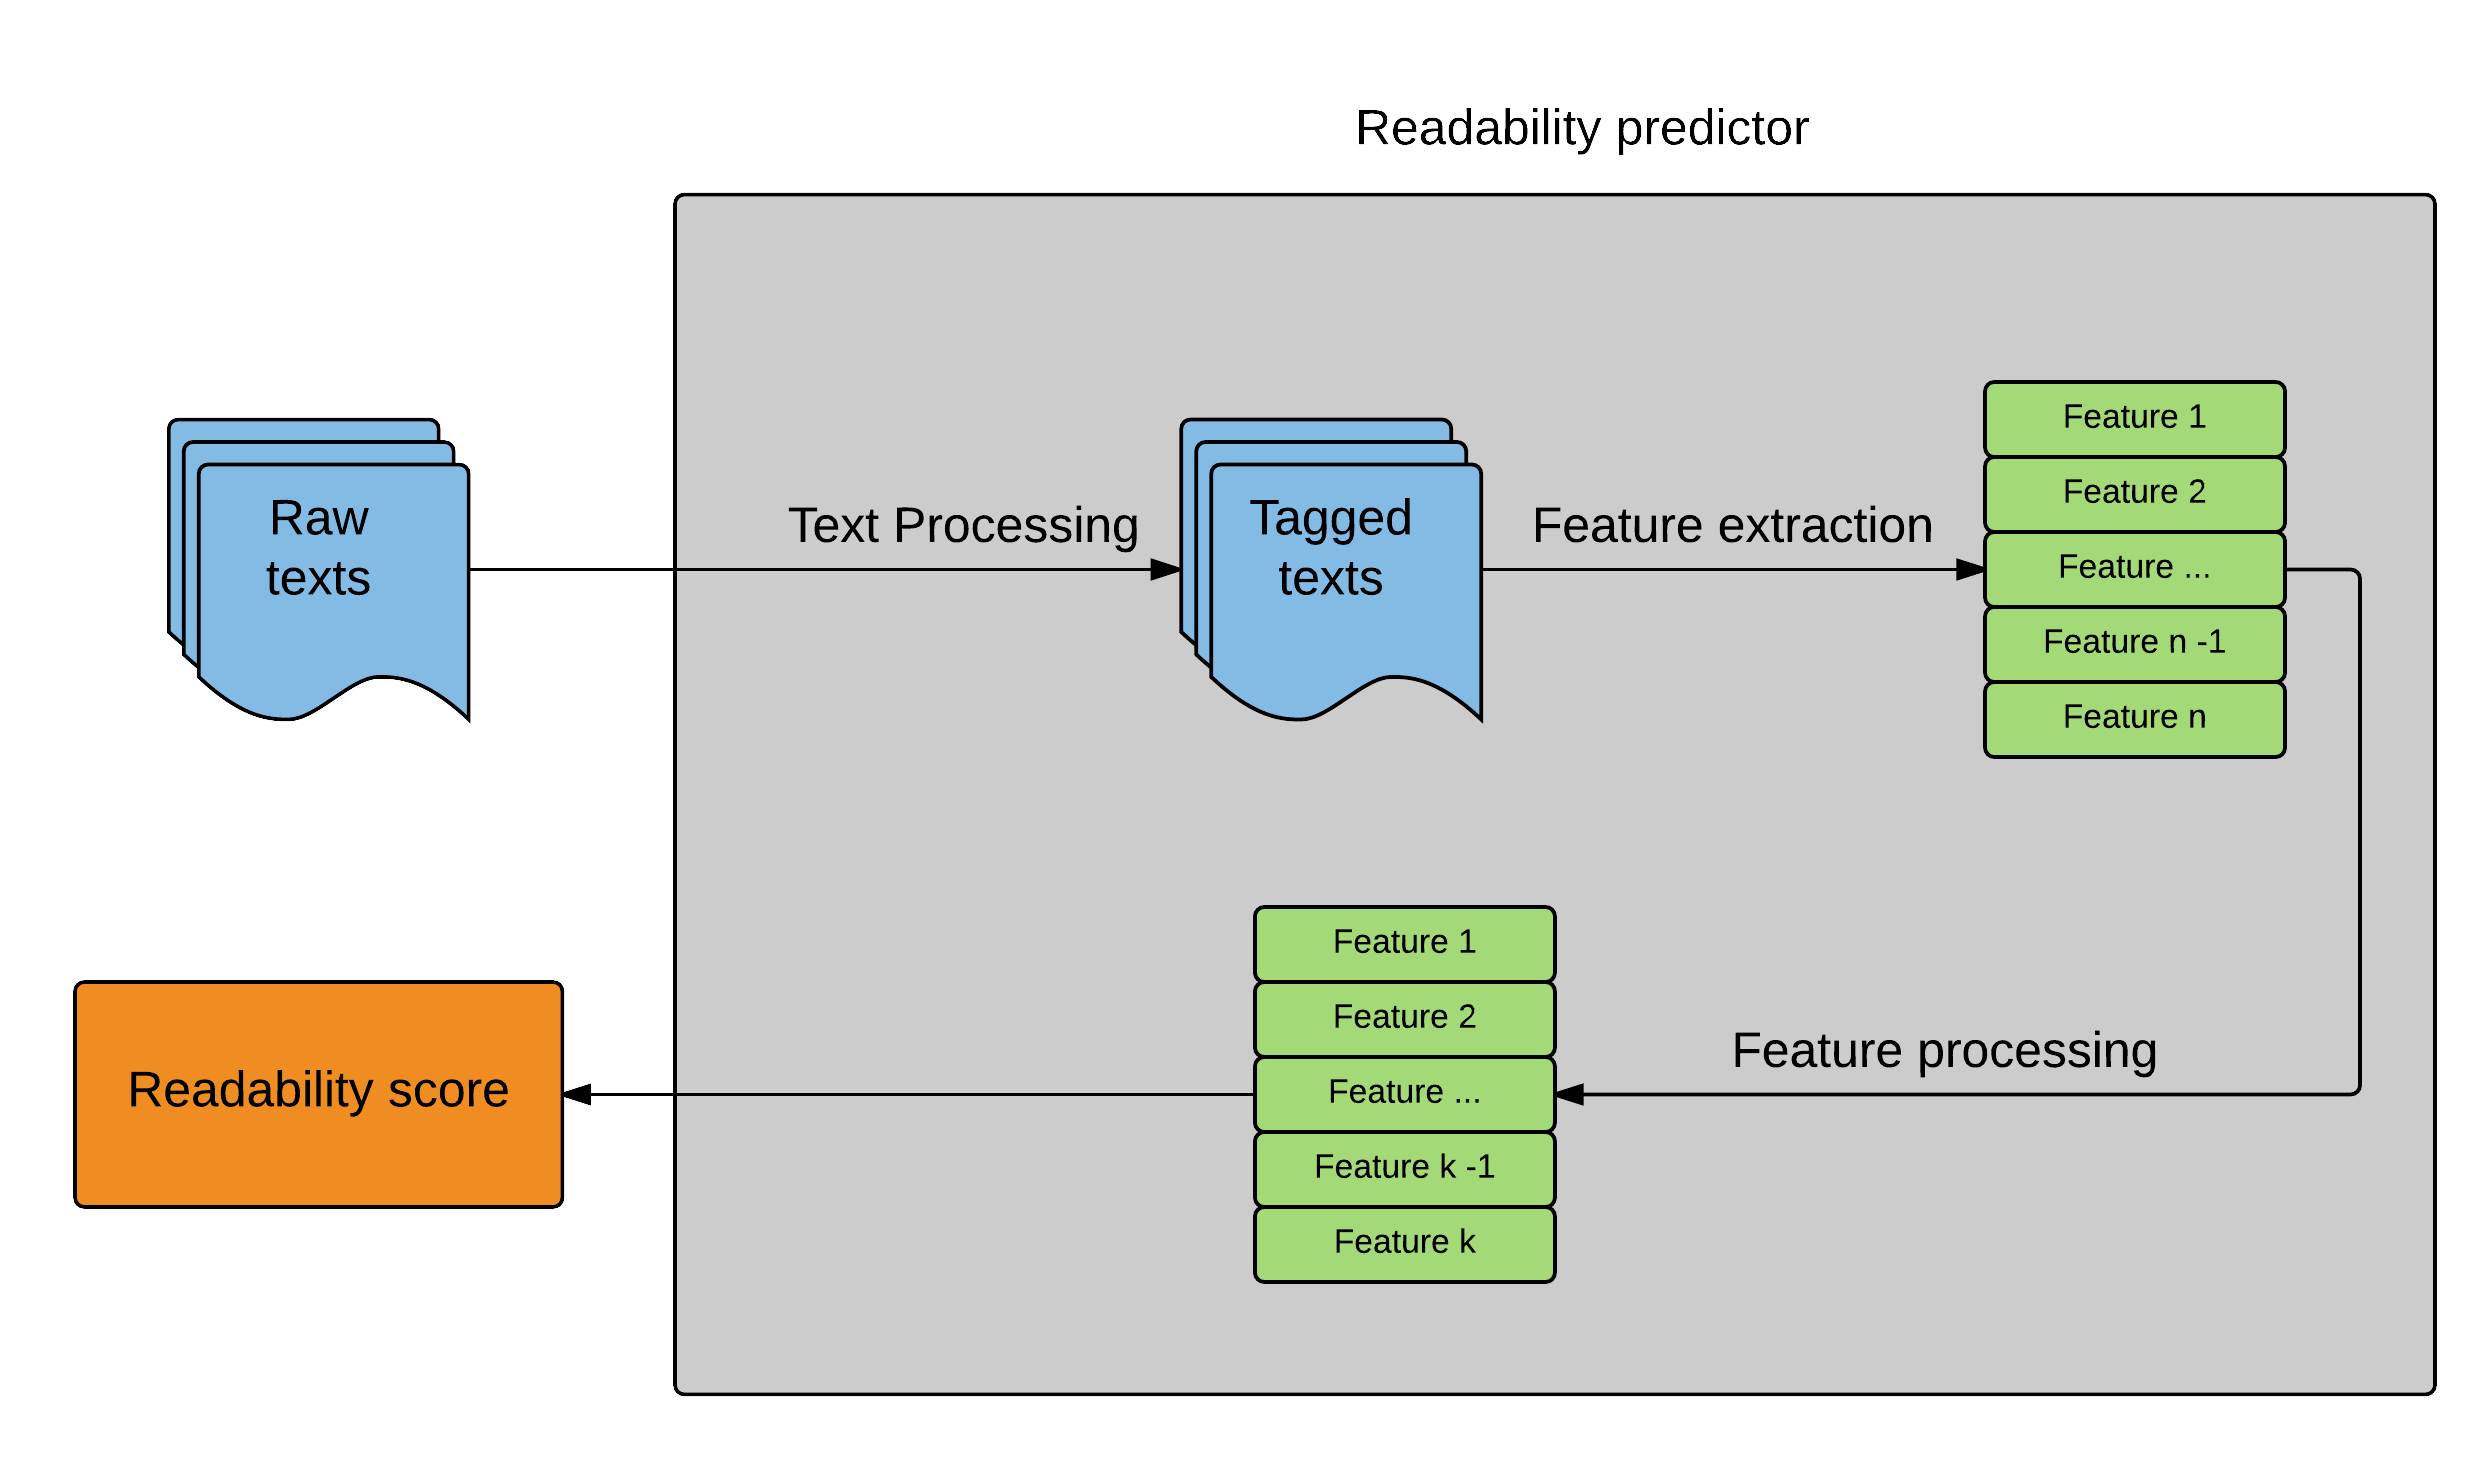
\includegraphics[width=\textwidth]{pipeline}
\caption{General pipeline}
\label{fig:pipeline}
\end{figure}

\subsection{Text processing}

The text processing step is the step where the raw text is given structure and, therefore, value. This structure and information will later be used for extraction features that will help the system predict a readability score.\\

The tool that has been chosen for natural language processing is Freeling NLP\cite{freelingNLP}. Freeling is an open source Natural language processing library that supports 11 different languages. The tool solves common NLP tasks, such as, Tokenization, sentence detection, Part of speech tagging or dependency parsing. Each of this processes will be helpful for building certain features later.\\

The \textbf{tokenization} is the base module for any NLP processing. Tokenization refers to taking a raw text and normalizing it into pieces that make text processing possible. This will also make possible, to implement tradition shallow features such as, Flesch–Kincaid \cite{flesch}. \\

The \textbf{Part of speech} analysis determines the function each token has in the sentence. This, together with \textbf{dependency parsing} techniques, make possible the analysis of syntactic structures in the sentences.\\

Other tools outside Freeling, such as \textbf{WordNet} or \textbf{Latent semantic analysis} techniques, will make possible to analyses texts at semantic level, for detecting structures that refer to concepts rather than to tokens themselves.\\


\subsection{Feature extraction}
This section describes the features proposed for the system. These features range from the most simple and commonly used ones such as the shallow features, to a more complex set of features such as the ones base on semantics.

\subsubsection*{Shallow features}
\subsubsection*{Part of Speech tags}

\subsubsection*{N-grams}

...

Description of all the features used. Why should this feature be valuable, give hypotheses and intuition behind the use of each feature. Give examples when needed.

\subsection{Feature processing and selection}
Describe algorithms used for feature processing and selection, why should they help get better results?

\subsection{Learning and prediction}
Describe algorithms for learning and prediction. Pros an cons of each algorithm, why should this algorithm adapt better to our problem?

\section{Evaluation}

\subsection{Datasets}
Information about how we get and extract the datasets.
\subsubsection{English}
\begin{itemize}
\item Lexile
\item List all for proposal...
\end{itemize}
\subsubsection{Spanish}
\begin{itemize}
\item Lexile
\item List all for proposal...
\end{itemize}
\subsubsection{Basque}
\begin{itemize}
\item Ikasbil
\end{itemize}

\subsection{Metrics}

\begin{itemize}
\item Error rate, accuracy
\item Adjacent accuracy, double adjacent accuracy...
\item Average error distance
\end{itemize}

\subsection{Tests}

\begin{itemize}

\item Which features add the most value? Correlation, information gain etc.

\item Do features correlate similarly with the readability score for each language?

\item Feature preprocessing, does it help?
	\begin{itemize}
	\item Discretization
	\item Feature subset selection techniques
	\end{itemize}
	
\item Comparison of learning models, which learning model fits best the problem?
	\begin{itemize}
	\item KNN
	\item Bayesian models
	\item SVM
	\item Neural network
	\item Regression (Adding a sense of order in class values)
	\item Ordinal classification (Adding a \textbf{stronger} sense of order in class values)
	\end{itemize}

\item \textbf{Comparison} of the system vs \textbf{baselines} such as fleish for each language individually.

\item Comparison \textbf{vs state of the art} systems for each language.

\item Multi vs monolingual
\item If we take a bilingual corpus, does the system predict same values? And if we take a text and translate it to another language? Does the readability values maintain using an automatic translator?
\end{itemize}



\bibliography{bibliography}{}
\bibliographystyle{plain}
\end{document}